\documentclass[a4paper]{article}

\usepackage{graphicx}
\usepackage{amsmath,amssymb}
\usepackage{minted}
\usepackage{multirow}
\usepackage{float}
\usepackage{todonotes}
\usepackage{forest}
\usepackage{xstring}
\usepackage{xcolor}
\usepackage[most]{tcolorbox}
\usepackage{xparse}
\usepackage{natbib}
\usepackage{tikz}

\usetikzlibrary{graphs,graphdrawing}
\usegdlibrary{layered}

% for external graphviz

\input{/home/donkarlo/Dropbox/repo/nd_language_ai_project/src/nd_language_ai/formal/computer/programming/tex/latex/code_clips/external_graphviz.tex}

% for tags

\input{/home/donkarlo/Dropbox/repo/nd_language_ai_project/src/nd_language_ai/formal/computer/programming/tex/latex/part/control_sequence/kind/semtag/semtag.tex}

% for links

\input{/home/donkarlo/Dropbox/repo/nd_language_ai_project/src/nd_language_ai/formal/computer/programming/tex/latex/code_clips/seehere.tex}

\title{Neural encoder training}

\date{}

\author{Mohammad Rahmani}

\begin{document}

   \maketitle

   \label{methodology_neural_encoder_tarining}

   %TODO add neural encoding citations

   Neural encoding training resembels kinematic teaching \cite{ablett-2025-multimodal-and-force-matched-imitation-learning-with-a-see-through-visuotactile-sensor} in which an expert agent teaches another agent how it should coordinate its sensory observations with its motor capabilities.

   in this section we discuss how to train the cognitive architecture we discussed in such that given a stimuli we learn both the temporal and hierarachical patter

   The sensory induction and perception is inspired from human nervous system in which each sensor plays the role of a sensory receptor and then in diverging neural circuits derived from each sensor, the sensor readings are converted to probability particles (= similar to neurotransmitters molcules that carry predetermined electrical loads in synapse clefts) to be equally devided between desired states as IPSP or EPSP graded potentials that gradually increase or decrease the state nuerion potential until that state neuron spikes to create an action potential.

   State neuron is a state in state space that we make an anlogy of it with neuron because similar to a neuron that receives neurotransmitters through its ion gates to convert them to graded IPSP or EPSP potentials, it converts a sensor reading to the positive or negative probability-like values to increase or decrease the probability up to the point that it reaches the threshold (similar to a neuron spike when its voltage reache -70v) and spikes and produces an action potential in two directions. One along the time axis in similar level and one along abstraction axis.

   In abstraction level the a pattern simllar to converging neural circuits is followed to reach a the highest abstraction.

   This language must be such that when a drone experiences something that it has not experienced in previous experiences then it should detect it as a from which it builds language.

   So we devide the experiment in two phases. In offline training phase, one robot(in this case a UAV equiped with LIDAR, GPS, IMU) is requested by human agent to use its autopilot to reach a set of trajectory points to gather sensory data from which temporal models and abstraction models using the aforementioned method inspired human nervous system is build.
   \section{Steps}
      \begin{figure}[H]
         \centering
         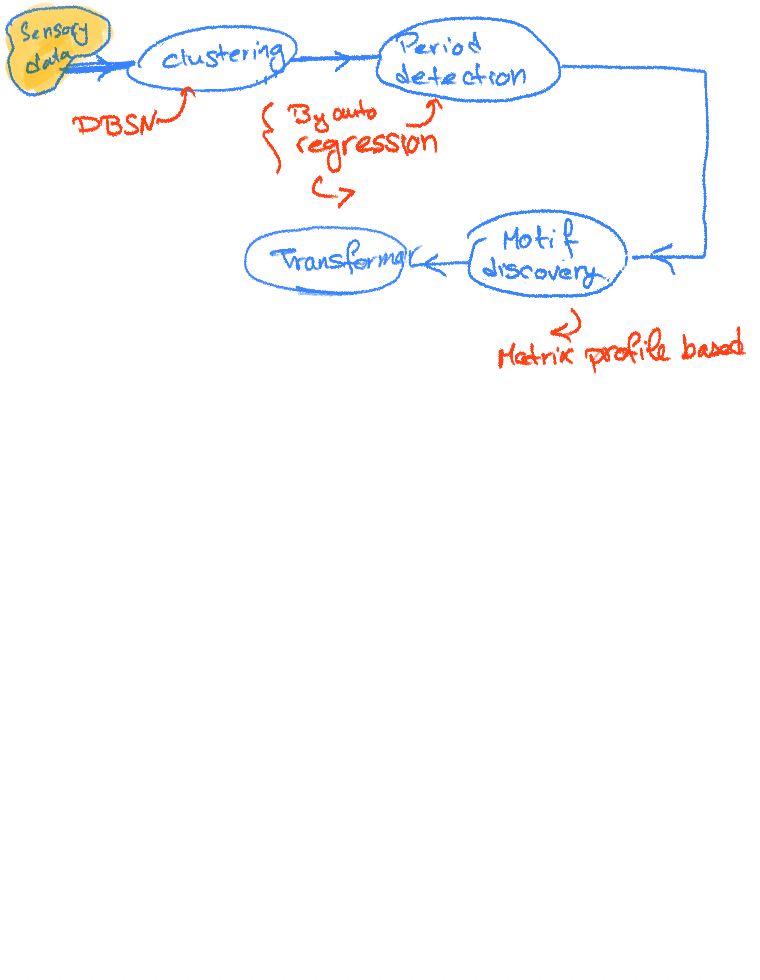
\includegraphics[width=0.9\textwidth]{training_steps.png}
      \end{figure}
      \subsection{Clustreing}
         Using density-based clustering method

      \subsection{Period detection with GRU based latent autocorollation fast fourier transform}
         \seeherefooter{/nd_datascience_learning_project/src/signal_processing/auto_correlation/fast_fourier_transform.tex}

         for implementation \seeherefooter{/repo/nd_datascience_project/src/nd_datascience/machine_learning/model/application/auto_correlation/sequence/period/neural/}

         The Fast Fourier Transform (FFT) is an autocorrolation method that efficiently converts a time-domain signal into its frequency components, allowing periodicity to be detected by identifying dominant frequencies corresponding to repeating patterns \cite{berberidis-2002-on-the-discovery-of-weak-periodicities-in-large-time-series}.

         A Gated Recurrent Unit (GRU) is a recurrent neural unit that uses reset and update gates to adaptively control how information is forgotten and retained across a sequence \cite{cho-2014-learning-phrase-representations-using-rnn-encoder-decoder-for-statistical-machine-translation}.

         The proposed period-discovery method first transforms the spike-train activity into a learned latent representation and then applies autocorrelation in the latent space. For each discrete interval, the observation-neuron firing rates are collected into

         \[
         \mathbf{q}_n
         =
         \operatorname{vec}_{i,d\in\{0,1\}}
         \left(
         r_{Z_i^{(d)}}([t_n,t_{n+1}])
         \right),
         \]

         where $r_{Z_i^{(d)}}([t_n,t_{n+1}])$ is the firing rate of observation neuron $Z_i^{(d)}$ during the corresponding interval.

         Overlapping windows of length $W$ are passed through a GRU autoencoder \cite{cho-2014-learning-phrase-representations-using-rnn-encoder-decoder-for-statistical-machine-translation}. The encoder produces a $K$-dimensional latent sequence

         \[
         \mathbf{h}_n
         =
         \mathcal{E}_{\phi}
         \left(
         \mathbf{q}_{n-W+1:n}
         \right),
         \]

         while the decoder $\mathcal{D}_{\psi}$ is trained to reconstruct the original window by minimizing

         \[
         (\phi^{*},\psi^{*})
         =
         \arg\min_{\phi,\psi}
         \sum_n
         \left\|
         \mathbf{q}_{n-W+1:n}
         -
         \mathcal{D}_{\psi}
         \left(
         \mathcal{E}_{\phi}
         \left(
         \mathbf{q}_{n-W+1:n}
         \right)
         \right)
         \right\|_2^2 .
         \]

         After training, overlapping latent representations are averaged to obtain one latent vector $\mathbf{h}_n$ for each time step. The multivariate latent autocorrelation at lag $\tau$ is then

         \[
         \rho_{\mathrm{GRU}}(\tau)
         =
         \frac{1}{n_{\max}-\tau}
         \sum_{k=1}^{K}
         \sum_{n=0}^{n_{\max}-\tau-1}
         h_{n,k}h_{n+\tau,k}.
         \]

         In the implementation, this autocorrelation is calculated efficiently using the Fast Fourier Transform,

         \[
         \rho_{\mathrm{GRU}}(\tau)
         =
         \frac{1}{n_{\max}-\tau}
         \sum_{k=1}^{K}
         \operatorname{IFFT}
         \left(
         \operatorname{FFT}(\mathbf{h}_{:,k})
         \overline{\operatorname{FFT}(\mathbf{h}_{:,k})}
         \right)_{\tau}.
         \]

         The estimated period is the first autocorrelation peak after a predefined minimum admissible lag $\tau_{\min}$,

         \[
         \hat{\tau}_{\mathrm{per}}
         =
         \min
         \left\{
         \tau \geq \tau_{\min}
         \mid
         \tau \text{ is a local maximum of }
         \rho_{\mathrm{GRU}}(\tau)
         \right\}.
         \]

         Thus, the GRU is not used to predict the period directly; it learns a latent representation in which repeated multivariate spike-train patterns can be detected by FFT-based autocorrelation.

         \begin{algorithm}[H]
            \caption{GRU-based latent autocorrelation for period discovery}
            \begin{algorithmic}[1]
               \State Construct firing-rate vectors $\mathbf{q}_n$ from the observation-neuron spike trains
               \State Form overlapping windows of length $W$
               \State Train a GRU autoencoder to reconstruct the input windows
               \State Encode all windows into latent sequences
               \State Average overlapping encodings to obtain one latent vector $\mathbf{h}_n$ per time step
               \State Compute multivariate autocorrelation of $\mathbf{h}_n$ using FFT
               \State Detect local maxima of $\rho_{\mathrm{GRU}}(\tau)$ for $\tau \geq \tau_{\min}$
               \State \Return the first detected peak as $\hat{\tau}_{\mathrm{per}}$
            \end{algorithmic}
         \end{algorithm}

      \subsection{Motif discovery}
         for general information \seeherefooter{/nd_math_learning_project/src/statistics/sequence/timeseries/motif_discovery/motif_discovery.tex}
         Here are two wellknown methods are introduced in
         \cite{guerrini-2025-time-series-motif-discovery-a-comprehensive-evaluation, linardi-2018-matrix-profile-x-valmod-scalable-discovery-of-variable-length-motifs-in-data-series}

         for the specific method used in this research
         \seeherefooter{/nd_math_learning_project/src/statistics/sequence/timeseries/motif_discovery/gru_autoencoder_based/gru_autoencoder_based.tex}
         and  \cite{linardi-2018-matrix-profile-x-valmod-scalable-discovery-of-variable-length-motifs-in-data-series}

         Motif discovery is performed independently at each representation level.

         For a selected representation level $\ell$, let

         \[
         \mathbf{s}_{\ell}
         =
         \left(
         s_{\ell,1},
         s_{\ell,2},
         \ldots,
         s_{\ell,N_{\ell}}
         \right)
         \]

         denote the ordered spike sequence generated by state neurons belonging to that level.

         A variable-length candidate subsequence is

         \[
         \mathbf{s}_{\ell}[a:b]
         =
         \left(
         s_{\ell,a},
         \ldots,
         s_{\ell,b}
         \right).
         \]

         A recurrent subsequence discovered at level $\ell$ is represented by the motif

         \[
         \mathbf{m}_{k,\ell}.
         \]

         A candidate subsequence is considered an occurrence of this motif when

         \[
         \Delta_{\ell}
         \left(
         \mathbf{s}_{\ell}[a:b],
         \mathbf{m}_{k,\ell}
         \right)
         \leq
         \varepsilon_{\ell},
         \]

         where $\Delta_{\ell}$ is the motif-distance function and
         $\varepsilon_{\ell}$ is the acceptance threshold used at representation level $\ell$.

         The same procedure is applied independently for every selected representation level,

         \[
         \ell \in L,
         \]

         without requiring information from either a lower or a higher representation level.

         \begin{algorithm}[H]
            \caption{Level-independent motif discovery}

            \begin{algorithmic}[1]
               \For{each selected representation level $\ell \in L$}
               \State Collect the spike sequence $\mathbf{s}_{\ell}$
               \State Generate variable-length candidate subsequences $\mathbf{s}_{\ell}[a:b]$
               \State Apply motif discovery to the sequence at level $\ell$
               \State Compare recurrent subsequences using $\Delta_{\ell}$
               \State Group subsequences satisfying the threshold $\varepsilon_{\ell}$
               \State Store each discovered recurrent pattern as a motif $\mathbf{m}_{k,\ell}$
               \EndFor

               \State Return the motifs discovered independently at each representation level
            \end{algorithmic}
         \end{algorithm}

   \section{Training Autoencoders, from ROS to potentials}
      This section biologically doesn't exist but it is explained here because the data for testing the framework is derived from Robot Operating system ni form of nested attriubte-value sensory data readings. As such a method is needed to simulate neunoral activity from this type of data.
      \begin{figure}[H]
         \centering
         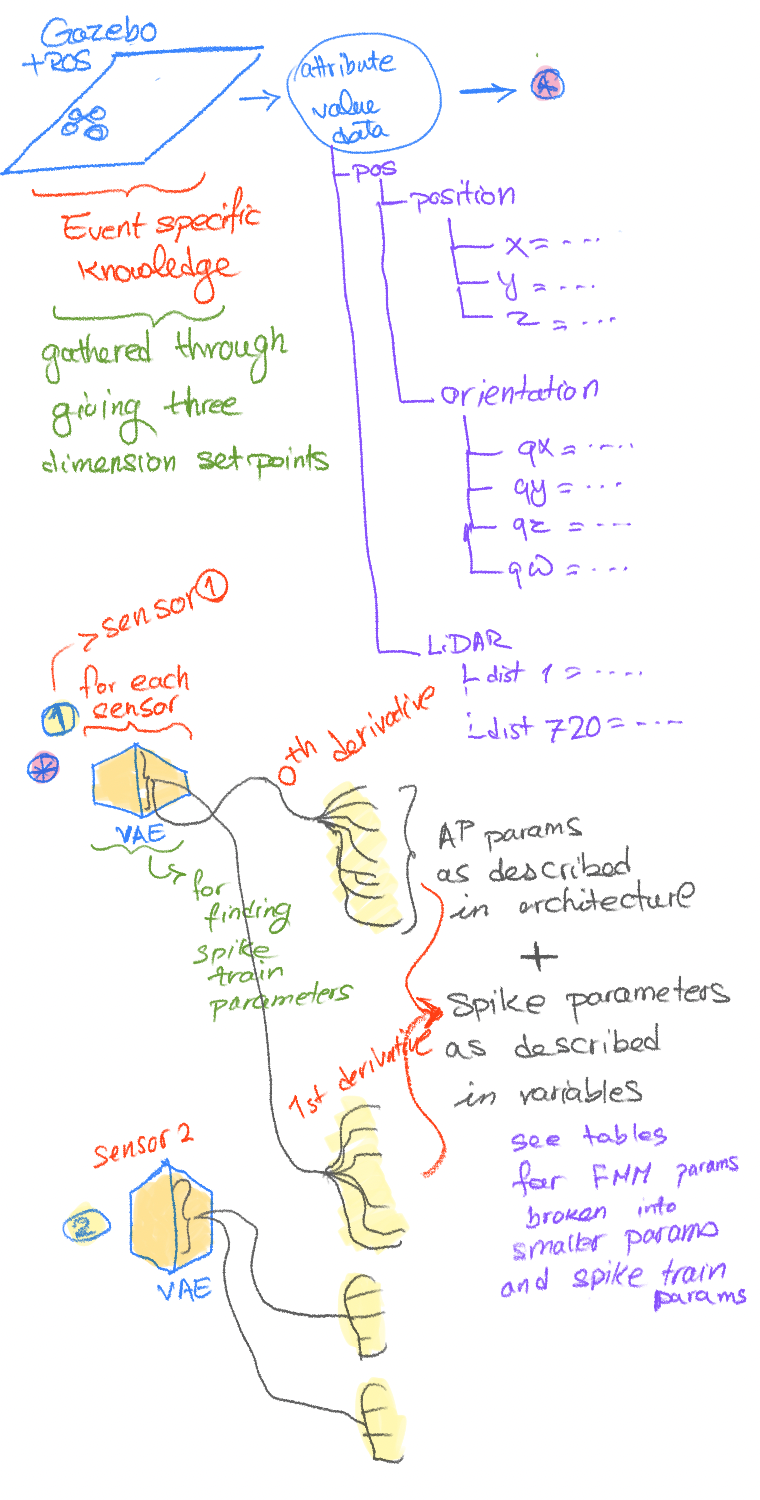
\includegraphics[width=0.9\textwidth]{ros_and_vae.png}
      \end{figure}

      This sections discusses how the structured data or traces from ROS messages are encoded to spike trains represented in FMM parameters using variational auto encoders.

      Using VAE for such encoding was used by other researchers too. \cite{shimazaki-2025-neural-coding-foundational-concepts-statistical-formulations-and-recent-advances} Transformation of neural activity to perception and behavior using combining classical concepts with statistical encoding and decoding frameworks.  \cite{granley-2022-hybrid-neural-autoencoders} proposes a Hybrid Neural Autoencoder in which a deep neural encoder learns stimulation patterns that produce desired neural or perceptual responses through a fixed biological forward model. The method is demonstrated for visual neuroprostheses and produces higher-fidelity patient-specific stimuli than conventional encoding strategies. see Figure 5 (bottom left shows for each number a new cluster is formed)

      \subsection{This research method}
         It is needed to develop a method that can follow the following rules to train a varational autoencoder

         \begin{itemize}
            \item The input is ROS yaml files from multiple sensor readings.  S we have multiple attribute-value or structured data readings
            \begin{itemize}
               \item from each sensor data we must pretend two esnsors exist.
               \begin{itemize}
                  \item A sensor that measures the intensity of the signal
                  \item Another sensor that measures the change rate of  previous sensor
               \end{itemize}
            \end{itemize}
            \item each of the aforementioned data points (nested attribute -value) should be converted to parameters of a spike train of action potentials using a variational autoencoder. These parameters are mentioned in Table \ref{table_action_potential_parameters} for an Action potential and in Table \ref{table_observation_neuron_spike_count_firing_rate} for a spike train. 
            \item the ranges for each of the above parameters for each sensors must be in non-confilicting intervals such that I can understand by seeing each value for each parameter, that from wich sensor or chage rate sensor it is derived. For spike train parameters, this rule doesn't apply to spike train perameters. 
            \item 

         \end{itemize}

   \section{Transformers}
      Since different segment composition of language form different meanings, LSTMs (and consequently RNNs) can not catch local dependencies. A multi attention predictor is needed. The transformers \cite{vaswani-2017-attention-is-all-you-need}

      Its application here is to replace the constant speed predictor

      \begin{itemize}
         \item At lowest level in each cell, it holds an AP wave represented by FMM
         \item Training
         \begin{itemize}
            \item Deep learning as an autocorrelation to find periods
         \end{itemize}
         \item Sliding windows to train the transformer
         \item Period sampling with auto corrlation for training and validating the transformer
         \item Noise as uncertainty in transformer

      \end{itemize}

      \subsection{Gaussain transformer}
         for all details \seeherefooter{/nd_datascience_learning_project/src/machine_learning/model/architecture/neural_network/kind/deep_learning/kind/transformer/kind/uncertainty/uncertainty.tex}

         The model receives a past time-series window and predicts a future window with uncertainty.

         \[
         f_{\theta}:
         \mathbb{R}^{T_{\mathrm{in}} \times F_{\mathrm{in}}}
         \rightarrow
         \mathbb{R}^{T_{\mathrm{out}} \times 2F_{\mathrm{out}}}
         \]

         For each future time step and feature, it predicts two values:

         \[
         \hat{Y}_{\mathrm{params}}
         =
         [
         \mu,
         \log \sigma^2
         ]
         \]

         \[
         y_{b,t,j}
         \sim
         \mathcal{N}
         (
         \mu_{b,t,j},
         \sigma^2_{b,t,j}
         )
         \]

         \begin{itemize}
            \item \(\mu\): expected future value
            \item \(\sigma^2 = \exp(\log \sigma^2)\): predictive uncertainty
         \end{itemize}

         \subsubsection{Loss and uncertainty calculation}
            The model is trained with Gaussian negative log-likelihood:

            \[
            \mathcal{L}
            =
            \frac{1}{BT_{\mathrm{out}}}
            \sum_{b=1}^{B}
            \sum_{t=1}^{T_{\mathrm{out}}}
            \sum_{j=1}^{F_{\mathrm{out}}}
            \frac{1}{2}
            \left[
            \log \sigma^2_{b,t,j}
            +
            (y_{b,t,j}-\mu_{b,t,j})^2
            \exp
            (
            -\log \sigma^2_{b,t,j}
            )
            \right]
            \]

            Approximate 95 percent prediction interval:

            \[
            y_{b,t,j}
            \in
            [
            \mu_{b,t,j}
            -
            1.96\sigma_{b,t,j},
            \mu_{b,t,j}
            +
            1.96\sigma_{b,t,j}
            ]
            \]

            \begin{itemize}
               \item Small variance means high confidence.
               \item Small variance means high confidence.
            \end{itemize}

   \section{Inputs for encoding training}

      \begin{itemize}

         \item Different sensor modalities

      \end{itemize}

   \section{Tasks by order in this phase}

      \begin{enumerate}

         \item Accumelating the sensory data from Robot Operating System
         \item training variational autoencoders to to break each sensory data into components action potential populations

         \item fusing different sensory modalities with variational autoencoders

         \item creating the the clusters for different levels

         \begin{itemize}

            \item here each sensory data already exists for sure in one of the clusters so wae can find the parameters from here after

         \end{itemize}

         \item Learning FMM psrameters for refractoring period for each state neuron at both concept axis and time axis

      \end{enumerate}

   \section{These items must be learned from these sensory data}

      All the parameters mentioned in in Arcitecture
      \begin{itemize}

         \item A probabilistic model based on Transformers for each level to predict sequences (This could be regarded as a sequential circuit). This probabilistic model will perform as grand modther neuron

         \item A probabilistic model for abstraction levels that maps a state neuron to the more abstract concepts by clustering

         \item A variational auto encoder to fuse all information together to assign an IPSP or EPSP value

         \item with what frequencey a sensory neuron should spike according to a stimuli

         \item Probabilistic dependency between different sensory modality (Spatial summation of graded potentials)

         \item Learning temporal summation distribution of graded potentials derived from multiple spikes

         \item Action potential parameters (and parameters for FMM)

         \begin{itemize}
            \item Maixmum potential or amplitutue or A in FMM
            \item spiking threshold
            \item Depolrization time period
            \item repolarization time period
            \item refractory time period
         \end{itemize}

         \item each EPSP and IPSP value

         \item The firing rate for both intensity and intensity change neurons.png

      \end{itemize}

   \section{Grand mother neurons that are used only in training phase}
      All the following method
      \subsection{Clustering neurons}
         Clusters data based on similarity of sensory data
         Based on DBSCAN (Density-Based Spatial Clustering of Applications with Noise)

         \documentclass[a4paper]{article}

\usepackage{graphicx}
\usepackage{amsmath,amssymb}
\usepackage{minted}
\usepackage{multirow}
\usepackage{float}
\usepackage{algorithm}
\usepackage{algpseudocode}
\usepackage{todonotes}
\usepackage{forest}
\usepackage{xstring}
\usepackage{xcolor}
\usepackage[most]{tcolorbox}
\usepackage{xparse}
\usepackage{natbib}
\usepackage{adjustbox}

\usetikzlibrary{graphs,graphdrawing}
\usegdlibrary{layered}

% for external graphviz
\input{/home/donkarlo/Dropbox/repo/nd_language_ai_project/src/nd_language_ai/formal/computer/programming/tex/latex/code_clips/external_graphviz.tex}

% for tags
\input{/home/donkarlo/Dropbox/repo/nd_language_ai_project/src/nd_language_ai/formal/computer/programming/tex/latex/part/control_sequence/kind/semtag/semtag.tex}

% for links
\input{/home/donkarlo/Dropbox/repo/nd_language_ai_project/src/nd_language_ai/formal/computer/programming/tex/latex/code_clips/seehere.tex}

% for nested lists and sections
\input{/home/donkarlo/Dropbox/repo/nd_language_ai_project/src/nd_language_ai/formal/computer/programming/tex/latex/code_clips/deep_structure.tex}

\title{Language building}
\date{}
\author{Mohammad Rahmani}

\begin{document}
   \maketitle
   \begin{figure}[H]
      \centering
      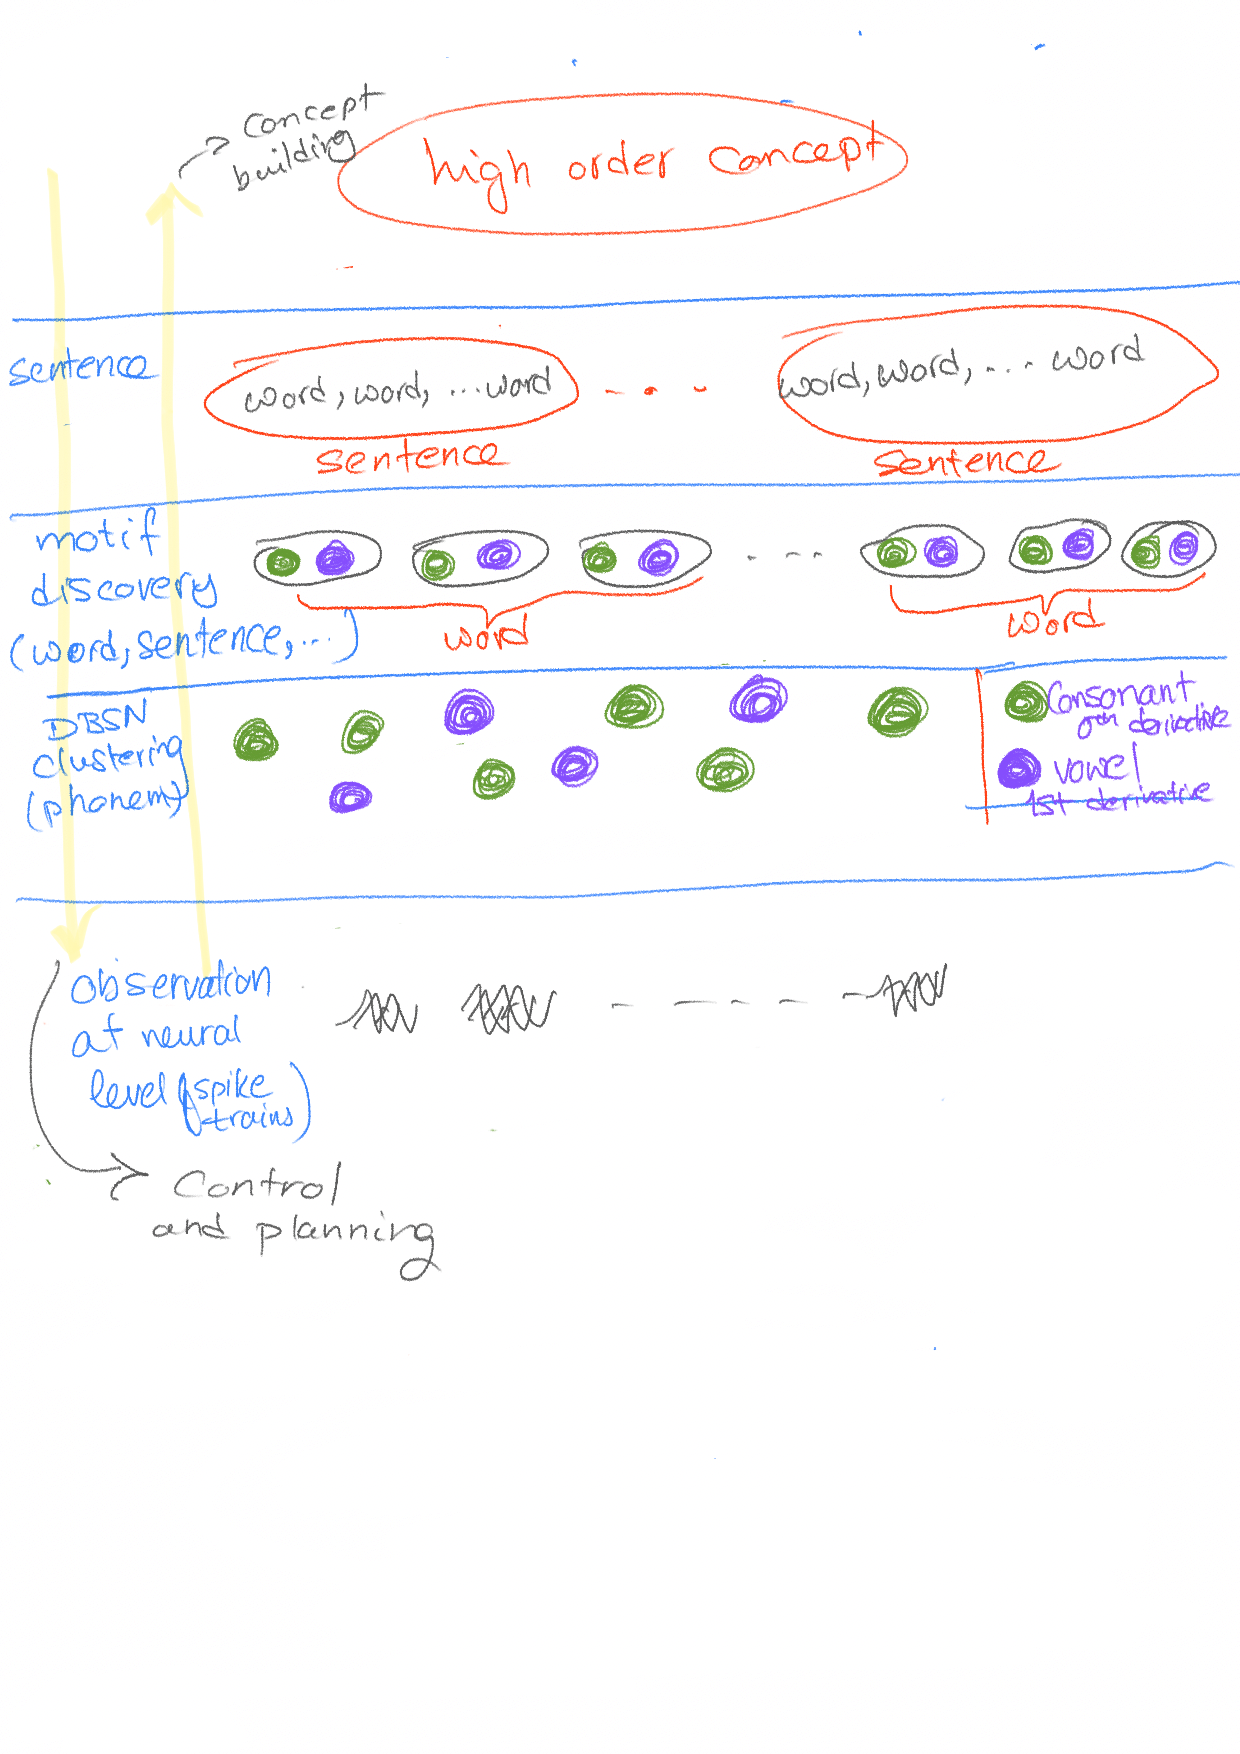
\includegraphics[width=0.9\textwidth]{language_building.png}
   \end{figure}
      \subsection{Motif discovery (to cluster timeseries)}
         In this research Matrix-Profile-based is used to cluster phonems to build words and to higher levels. This is explained in language section .

         \seeherefooter{/home/donkarlo/Dropbox/repo/nd_math_learning_project/src/statistics/sequence/timeseries/motif_discovery/matrix_profile_based/matrix_profiled_based.tex}
         To discover the periodic data. As we will see in the experiment section a drone that circules a rectangualar corridor makes many periodic sensory data that motif discovery is used for it. Then a method is needed to find the cycles in sensory data.

         This research uses Matrix-Profile-based  method for this .

         This method doesn't need training.
         \textbf{Matrix-Profile-based Motif Discovery \cite{vanonsem-2023-variable-length-motif-discovery-in-time-series-data}}
         \begin{algorithm}[H]
            \caption{Event-Driven Variable-Length Motif Discovery}
            \begin{algorithmic}[1]
               \State Input time series \(T\), window size \(w\), threshold \(t\)
               \State Compute scale-aware distance matrix \(M\)
               \State Convert \(M\) to binary event matrix \(M_{\mathrm{bin}}\)
               \State Rank diagonals of \(M_{\mathrm{bin}}\) by number Weightof events
               \For{each ranked diagonal}
               \For{each event on the diagonal}
               \State Enlarge the event into a motif candidate
               \State Validate candidate using the distance threshold
               \State Find all occurrences of the accepted motif
               \State Add motif and its occurrences to output
               \State Exclude found occurrences from \(M_{\mathrm{bin}}\)
               \EndFor
               \EndFor
               \State Return unique motifs with grouped occurrences
            \end{algorithmic}
         \end{algorithm}
         \bibliographystyle{plainnat}
         \bibliography{/home/donkarlo/Dropbox/repo/nd_shared_research/bibliography/bibliography.bib}
\end{document}


         \bibliographystyle{plainnat}

         \bibliography{/home/donkarlo/Dropbox/repo/nd_shared_research/bibliography/bibliography.bib}

\end{document}